\documentclass[a4paper,12pt,oneside]{book}
\usepackage{pdfpages}
\usepackage{polski}
\usepackage{fancyhdr}
\usepackage{graphicx}
\usepackage{pgf-pie}
\usepackage{float}
\usepackage{caption}
\usepackage{subcaption}

\linespread{1.25}
\pagestyle{fancy}
\fancyhf{}
\fancyhead[LO]{\footnotesize\rightmark}
\fancyhead[RE]{\footnotesize\leftmark}
\fancyhead[LE,RO]{\footnotesize\thepage}
\begin{document}
	\thispagestyle{empty}
	\includepdf{stronatytulowa}
	
	\newpage
	\thispagestyle{empty}
	\chapter*{Streszczenie}
		Lorem ipsum dolor sit amet, consectetur adipiscing elit. Mauris nec neque urna. Morbi eu ante id quam pretium ultrices eget a nulla. Nulla lorem mi, laoreet vitae rutrum tempor, venenatis a sem. Donec dignissim ex quis varius commodo. Ut vel diam volutpat nisl convallis venenatis. Quisque tincidunt interdum tellus, eu rhoncus purus rhoncus ut. Cras rhoncus porttitor mollis.
	
		Vivamus ornare, sem sit amet dignissim vestibulum, velit libero congue est, at varius tellus tortor eget libero. Praesent egestas vel est in accumsan. Fusce vehicula sapien auctor, vehicula tellus id, bibendum est. Proin eu metus at sapien porttitor lobortis sit amet pellentesque ex. Ut maximus dui non sagittis ultrices. Duis sem massa, pulvinar vitae vulputate fermentum, vehicula at mauris. Morbi luctus vel quam ut sagittis. Mauris sollicitudin non purus vel dictum. Aenean facilisis eget mi non feugiat. Class aptent taciti sociosqu ad litora torquent per conubia nostra, per inceptos himenaeos. Integer bibendum tellus vitae ex facilisis mollis. Proin iaculis auctor pulvinar. Suspendisse potenti.
			
		\textbf{Słowa kluczowe:} \textit{aplikacja mobilna, rolnictwo, react native}
	
		\newpage
	\thispagestyle{empty}
	\chapter*{Abstract}
		Lorem ipsum dolor sit amet, consectetur adipiscing elit. Mauris nec neque urna. Morbi eu ante id quam pretium ultrices eget a nulla. Nulla lorem mi, laoreet vitae rutrum tempor, venenatis a sem. Donec dignissim ex quis varius commodo. Ut vel diam volutpat nisl convallis venenatis. Quisque tincidunt interdum tellus, eu rhoncus purus rhoncus ut. Cras rhoncus porttitor mollis.
	
		Vivamus ornare, sem sit amet dignissim vestibulum, velit libero congue est, at varius tellus tortor eget libero. Praesent egestas vel est in accumsan. Fusce vehicula sapien auctor, vehicula tellus id, bibendum est. Proin eu metus at sapien porttitor lobortis sit amet pellentesque ex. Ut maximus dui non sagittis ultrices. Duis sem massa, pulvinar vitae vulputate fermentum, vehicula at mauris. Morbi luctus vel quam ut sagittis. Mauris sollicitudin non purus vel dictum. Aenean facilisis eget mi non feugiat. Class aptent taciti sociosqu ad litora torquent per conubia nostra, per inceptos himenaeos. Integer bibendum tellus vitae ex facilisis mollis. Proin iaculis auctor pulvinar. Suspendisse potenti.
		
		\textbf{Keywords:} \textit{mobile application, farming, react native}
	
	\newpage
	\thispagestyle{empty} %usuń styl (fancyheader)
	\tableofcontents %spis tresci
	
	\newpage
	\thispagestyle{empty}
	\chapter*{Wstęp} %bez numeru
	Lorem ipsum dolor sit amet, consectetur adipiscing elit. Mauris nec neque urna. Morbi eu ante id quam pretium ultrices eget a nulla. Nulla lorem mi, laoreet vitae rutrum tempor, venenatis a sem. Donec dignissim ex quis varius commodo. Ut vel diam volutpat nisl convallis venenatis. Quisque tincidunt interdum tellus, eu rhoncus purus rhoncus ut. Cras rhoncus porttitor mollis.
	
	Vivamus ornare, sem sit amet dignissim vestibulum, velit libero congue est, at varius tellus tortor eget libero. Praesent egestas vel est in accumsan. Fusce vehicula sapien auctor, vehicula tellus id, bibendum est. Proin eu metus at sapien porttitor lobortis sit amet pellentesque ex. Ut maximus dui non sagittis ultrices. Duis sem massa, pulvinar vitae vulputate fermentum, vehicula at mauris. Morbi luctus vel quam ut sagittis. Mauris sollicitudin non purus vel dictum. Aenean facilisis eget mi non feugiat. Class aptent taciti sociosqu ad litora torquent per conubia nostra, per inceptos himenaeos. Integer bibendum tellus vitae ex facilisis mollis. Proin iaculis auctor pulvinar. Suspendisse potenti.
	\addcontentsline{toc}{chapter}{Wstęp}
	
	\newpage
	\thispagestyle{empty}
	\chapter{Urządzenia mobilne}
	\section{Początki urządzeń mobilnych}
	Nie da się ukryć, że w dzisiejszych czasach wszelka technologia rozwija się w zawrotnym tempie. W przeciągu ostatnich siedmiu dekad na rynek wchodziły coraz nowsze urządzenia elektroniczne mające na celu ułatwienie dostępu do informacji oraz do kontaktu między ludźmi. Pierwsze prototypy telefonów komórkowych zaczęły się pojawiać w latach pięćdziesiątych dwudziestego wieku, kiedy to szwedzka firma Ericson zaprezentowała pierwszy przenośny telefon ważący około 40 kilogramów, a kształtem przypominający walizkę. W 1973 roku firma Motorola wprowadziła do sprzedaży Motorolę DynaTAC 8000X. Telefon ten porównać można było do cegły głownie przez jego wagę oraz rozmiar, a wzorowany był na urządzeniu używanym przez bohatera popularnej serii "Star Trek". Urządzenie niczym nie przypominało telefonów produkowanych w dzisiejszych czasach. Jego bateria wystarczyła na zaledwie 30 minut rozmów, a naładowanie go trwało około 10 godzin. Przez następne lata, na rynek trafiały coraz to nowsze urządzenia oraz technologie produkowane przez firmy takie jak: Nokia, IBM, Motorola czy Siemens. Początki dwudziestego pierwszego wieku to okres w którym urządzenia mobilne przeszły w nową epokę, a mowa tu dokładniej o pierwszych telefonach dotykowych.
	
	\section{Pierwsze smartfony}
	Smartfon to inaczej przenośne urządzenie posiadające w sobie funkcje telefonu komórkowego oraz komputera osobistego. Pierwsze pomysły na ich stworzenie pojawiły się w 1992 roku. Prototyp takiego urządzenia został zaprezentowany przez firmę IBM. Pozwalał on na prowadzenie rozmów, wysyłanie faxów i poczty elektronicznej oraz przeglądanie stron internetowych. Było to dosyć prymitywne urządzenie o dużych rozmiarach. Prawdziwym przełomem okazał się rok 2007, kiedy to 9 stycznia firma Apple zaprezentowała swój pierwszy iPhone, który zawitał na rynku pół roku później.
	
	\begin{figure}[h]
		\centering
		\includegraphics[width=0.75\textwidth]{grafika/steve_jobs_iphone_presentation.png}
		\caption{Steve Jobs prezentujący pierwszy model iPhone}
	\end{figure}
	
	Wprowadzenie iPhone na rynek był gigantycznym skokiem w technologii. Ciężko było w jakikolwiek sposób z nim konkurować, ponieważ urządzenie to swoją konstrukcją, prostotą użycia oraz funkcjonalnościami przyćmiewała inne urządzenia. Producenci zrezygnowali z dosyć popularnych funkcjonalności, które były popularne w tamtych czasach. Klawiaturę zastąpiono ekranem dotykowym, a samo urządzenie posiadało 3,5 calowy ekran oraz przycisk "Home". 
	\newpage
	Na dzień premiery iPhone posiadał wiele więcej rewolucyjnych funkcjonalności takich jak:
	
	\begin{description}
		\item[Klawiatura ekranowa -] pozwalającą na wprowadzanie danych przez klawiaturę używając ekranu dotykowego. Funkcja ta posiadała również korektę dotknięć, która ignorowała przypadkowe kliknięcia na ekranie.
		\item[Czujnik zbliżeniowy -] który wyłączał ekran podczas gdy użytkownik zbliżył twarz do ekranu urządzenia.
		\item[Nowoczesna przeglądarka internetowa -] która pozwalała na wykorzystanie pełni możliwości języka HTML.
		\item[Multitouch -] czyli możliwość wykrywania przez ekran dotykowy wielu jednoczesnych kliknięć.
		\item[Żyroskop -] czyli funkcja wykrywająca stopień pochylenia urządzenia. 
	\end{description}

	Kolejne lata można nazwać "wyścigiem technologicznym", w którym to firmy konkurowały ze sobą tworząc coraz nowsze urządzenia oraz rozwijały istniejące już technologie w celu dorównania do wymogów konsumentów.
	
	\begin{figure}[h]
		\centering
		\includegraphics[width=0.75\textwidth]{grafika/iphone11}
		\caption{Model iPhone 11 wydany w 2019r}
	\end{figure}
	
	\newpage
	\section{Smartfony w dzisiejszych czasach}
	Dziś, liczba producentów na rynku produkujących urządzenia mobilne jest spora i dalej rośnie. W ciągu ostatnich piętnastu lat pojawiali się nowi producenci smartfonów razem ze swoimi innowacyjnymi pomysłami ulepszającymi swoje poprzednie urządzenia. 
	
	\begin{figure}[h]
		\centering
		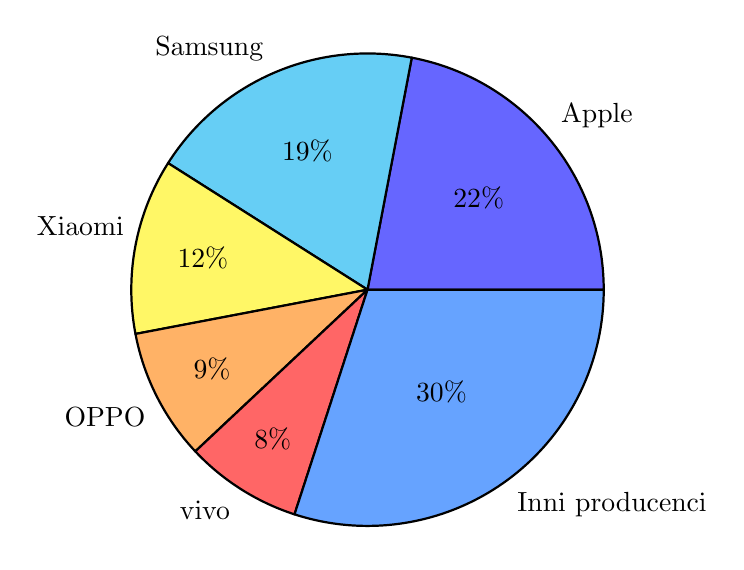
\begin{tikzpicture}
			\pie[radius=3]{22/Apple,
				19/Samsung,
				12/Xiaomi,
				9/OPPO,
				8/vivo,
				30/Inni producenci}
		\end{tikzpicture}
		\caption{Udział w globalnym rynku dostaw smartfonów, 4 kwartał 2021r}
	\end{figure}
	
	Jak widać na załączonym wyżej wykresie, globalnym liderem rynkowym nadal pozostaje Apple wraz ze swoim flagowym produktem iPhone. Na drugim i trzecim miejscu utrzymują się firmy Samsung oraz Xiaomi. Można więc wywnioskować, że wzrost liczby producentów oraz urządzeń dostępnych na rynku jak i coraz niższe ceny telefonów, przekładają się na korzystniejszą dostępność oraz większą popularność danych modeli. W wynikach badań przeprowadzonych przez CBOS (Centrum Badania Opinii Społecznej) z 2021 roku, w których sprawdzano jak na przestrzeni lat zmieniała się popularność telefonów posiadanych w polskich gospodarstwach domowych, zauważyć można owe zmiany w popularności urządzeń mobilnych.
	
	\newpage
	\begin{figure}[h]
		\centering
		\includegraphics[width=0.75\textwidth]{grafika/cbos_wykres}
		\caption{Telefony w gospodarstwach domowych w latach 1996-2017}
	\end{figure}

	Jak widać na przedstawionym wykresie, urządzenia mobilne zaczęły dosyć szybko stawać się popularne. Początkiem popularności telefonów komórkowych nad telefonami stacjonarnymi był rok 2007, kiedy to, jak już wcześniej było wspomniane, do sprzedaży wprowadzono pierwszy model iPhone. Rok ten można nazwać początkiem ery nowych urządzeń mobilnych. Sam wybór między klasycznym telefonem komórkowym, a smartfonem jest w głównej mierze uwarunkowany wiekiem i grupą społeczną użytkownika.
	
	\begin{figure}[h]
		\centering
		\includegraphics[width=1\textwidth]{grafika/cbos_wykres2}
		\caption{Procent wyboru klasycznych telefonów komórkowych i smartfonów w różnych przedziałach wiekowych}
	\end{figure}

	\newpage

	Powyższa tabela pokazuje preferencje wyboru telefonów wśród użytkowników względem ich wieku. Dla osób w wieku od 18 do 24 lat najbardziej popularne są smartfony. Liczba ta z każdą kategorią wiekową maleje. Dzieje się tak dlatego, że młodsze społeczeństwo jest bardziej przyswojone do zmian i nowości technologicznych, w przeciwieństwie do starszego społeczeństwa.
	
	\section{Smartfony i inne technologie używanie w rolnictwie}
	Jak już wcześniej zostało to wspomniane, jednymi z głównych czynników w tym czy dana osoba chętniej korzysta z urządzeń mobilnych jest wiek oraz grupa społeczna. Wśród najczęstszych posiadaczy smartfonów można wyróżnić studentów, uczniów szkół, pracowników biurowych oraz specjalistów z wyższym wykształceniem. Można więc dojść do wniosku, że urządzenia typu smartfon w większości są używane przez osoby kształcące się oraz przez osoby wykonujące pracę umysłową. Rolnicy natomiast są zaliczani do grupy osób wykonujących prace czysto fizyczną. Większość osób uważa rolników za osoby nie posiadające większej wiedzy na temat nowoczesnych technologii. Nic bardziej mylnego. Na przełomie ostatnich lat, rolnictwo ewoluowało i przyswajało coraz to nowsze technologie. Można powiedzieć, że smartfony stały się podstawowym narzędziem rolników. Dzięki nim rolnicy są w stanie używać nowych technologii takich jak:
	
	\begin{description}
		\item[Drony -] sterowane za pomocą telefonów, pozwalają na doglądanie upraw z lotu ptaka, tworzenia precyzyjnych map pól, a nawet nawożenie upraw środkami do ochrony roślin.
		\item[Czujniki upraw -] które ułatwiają kontrolę upraw oraz pozwalają na skuteczne dawkowanie nawozów.
		\item[GPS -] przy pomocy którego można dokumentować stan gruntów rolnych oraz mapować pola.
		\item[Aplikacje mobilne -] pozwalają one na łatwe zarządzanie gospodarstwem za pomocą smartfonów. Rolnik może używać ich w każdej chwili, przechowywać ważne informacje, używać ich do sprawdzania warunków pogodowych, robić notatki, planować pracę oraz wiele więcej.
	\end{description}

	Zmiany te są bardziej widoczne wśród młodszych rolników, którzy chętniej przyswajają nowe technologie, aby dzięki nim osiągnąć lepsze wyniki produkcji, ułatwić sobie wykonywaną pracę oraz zaoszczędzić sporo czasu.
	
	\newpage
	\thispagestyle{empty}
	\chapter{Systemy i aplikacje mobilne}
	\section{Mobilne systemy operacyjne}
	Sama nazwa "system operacyjny" kojarzona jest głównie z komputerami osobistymi. Systemy mobilne mimo tego, że w pewnym stopniu bazują na systemach operacyjnych używanych w komputerach osobistych to posiadają szereg różnic i usprawnień stworzonych głównie w celu ułatwienia użytkownikowi w posługiwaniu się urządzeniem. Szybki rozwój urządzeń mobilnych przyczynił się do stworzenia systemów takich jak Symbian, Windows Phone, BlackBerry OS, iOS czy Android, z których to właśnie te dwa ostatnie czyli iOS oraz Android są liderami używanymi w dzisiejszych czasach.
	
	\subsection{System iOS}
	System iOS jest systemem stworzonym oraz w dalszym ciągu rozwijanym przez firmę Apple dostępnym tylko na urządzeniach tej firmy. Początkowo nazywany iPhone OS, system ten po raz pierwszy został zaprezentowany w roku 2007 przez Steava Jobsa podczas prezentacji pierwszego iPhone. System iOS bazuje na architekturze systemu Mac OS X, a ich struktura składa się z czterech abstrakcyjnych warstw.
	
	\newpage
	
	\begin{figure}[h]
		\centering
		\includegraphics[width=0.85\textwidth]{grafika/warstwy_ios.png}
		\caption{Warstwy systemu iOS}
	\end{figure}

	Pierwsza warstwa, czyli "Cocoa Touch" jest biblioteką odpowiedzialną za interfejs użytkownika. Interfejs ten jest sterowany za pomocą wbudowanego ekranu dotykowego. Warstwa "Media" jest warstwą obsługującą dźwięk i obraz. W skład tej warstwy wchodzą biblioteki takie jak: OpenGLES, Quartz, Core Graphics, Core Audio, Open AL oraz Media Player. Kolejną warstwą wchodzącą w skład systemu iOS jest warstwa "Core Services". Odpowiada ona za zarządzanie aplikacjami oraz wątkami. Posiada także funkcje obsługujące sieć i bazy danych. Ostatnią z warstw jest warstwa "Core OS", która ma za zadanie zapewnienia komunikacji między urządzeniem, a oprogramowaniem. Z biegiem lat powstawały nowe wersje systemu, które posiadały szereg udogodnień oraz poprawek. Obecnie istnieje szesnaście wersji systemu iOS. 
	
	\subsection{System Android}
	W roku 2005 po przejęciu przez firmę Google firmy Android Inc, stworzony został system na urządzenia mobilne oparty na jądrze Linuxa o nazwie Android. Prototypy urządzeń wraz z systemem zostały zaprezentowane w 2008 roku na Mobile World Congres. Od tamtej pory rozwój systemu Android przyśpieszył, aby następnie w 2013 roku zostać ogłoszonym najpopularniejszym systemem mobilnym na świecie.
	
	\newpage
	Schemat systemu Android prezentuje się następująco na rysunku 2.2.
	
	\begin{figure}[h]
		\centering
		\includegraphics[width=0.70\textwidth]{grafika/schemat_android.png}
		\caption{Schemat systemu Android}
	\end{figure}
	
	System Android cechuje się wieloma zaletami z których najważniejszymi są elastyczność systemu, intuicyjność obsługi, mnogość nakładek systemowych, regularne aktualizacje systemowe oraz możliwość rootowania urządzenia i wrzucenia dowolnego systemu. System ten posiada również kilka wad z których największą z nich jest duża podatność na ataki. Patrząc na dzisiejszy rynek telefonów, system Android jest zdecydowanym liderem pod względem dostępności. W przeciwieństwie do systemu iOS, który jest dostępny wyłącznie na urządzeniach firmy Apple, Android jest systemem dostępnym na urządzeniach wielu różnych producentów.
	
	\section{Rozwój aplikacji mobilnych}
	Aplikacje mobilne to rodzaj oprogramowania tworzonego z myślą o urządzeniach mobilnych. Aplikacje te podzielić można na podstawie ich zastosowania oraz grupy osób dla której zostały one stworzone. Zdecydowanie najpopularniejszymi typami aplikacji mobilnych są aplikacje społecznościowe.
	
	\begin{figure}[h]
		\centering
		\includegraphics[width=0.9\textwidth]{grafika/most_popular_apps_2021.png}
		\caption{Lista najpopularniejszych aplikacji mobilnych w 2021 roku pod względem ilości pobrań}
	\end{figure}

	Jak widać na załączonym rysunku 2.3 w pierwszej dziesiątce, aż osiem pozycji to aplikacje społecznościowe.  W ciągu ostatnich lat oprogramowanie mobilne ewoluowało wraz z dostępnymi na rynku urządzeniami. Wprowadzanie przez producentów nowych funkcjonalności do swoich urządzeń dawało deweloperom aplikacji na smartfony coraz większe możliwości. 
	
	\newpage
	
	Oprócz zmian na rynku aplikacji oraz urządzeń mobilnych z biegiem lat można było zauważyć powstawanie nowych środowisk skierowanych dla programistów aplikacji mobilnych. Do tych najpopularniejszych możemy zaliczyć: Flutter, Ionic, VueJS, Mobile Angular UI, Xamarin, jQuery Mobile, NativeScript, React Native. Używają one różnych języków programowania takich jak C/C++ w przypadku Flutter, JavaScript dla React Native, VueJS i jQuery Mobile, czy C-sharp w Xamarin. Większość tych frameworków wspiera wieloplatformowość, gdzie aplikacje pisane są głównie z myślą o urządzeniach z Androidem oraz iOS.
	
	\section{Aplikacje dla rolników}
	Celem tej pracy jest przedstawienie aplikacji zaprojektowanej dla rolników, dlatego nie może tu zabraknąć wzmianek o oprogramowaniu oraz rozwiązaniach dostępnych na rynku. W serwisach takich jak "Sklep Play" w łatwy sposób pobrać możemy aplikacje dla rolników które posiadają w sobie funkcje takie jak: menadżer pola, który pozwala użytkownikowi na oznaczanie oraz zapisywanie na mapach swoich pól, aplikacje typu kalkulator, które pozwalają na obliczanie wskaźników wysiewu czy stóp kapitalizacji, aplikacje z wyszukiwarkami chorób i środków ochrony roślin. Funkcje wymienione wyżej są jednymi z najczęściej używanych funkcjonalności w aplikacjach rolniczych.
	
	Zdecydowanie najczęściej pojawiającym się typem aplikacji w Sklepie Play, w kategorii "rolnictwo" jest nawigacja dla rolników. Przykładem takiej aplikacji jest "Nawigator polowy". Aplikacja ta pozwala na tworzenie listy posiadanych pól oraz zarządzanie nimi. Przy użyciu map Google użytkownik może znaleźć po swojej aktualnej lokalizacji lub po przez wpisanie adresu miejsce w którym pole może się znajdować. Następnie, tak jak jest to przedstawione na rysunku 2.4, użytkownik jest w stanie zaznaczyć obszar rolny na mapie, nazwać go i określić jaka uprawa się na nim znajduje. Po zapisaniu, pole zostanie dodane do listy wraz z jego opisami oraz powierzchnią. Tam rolnik jest w stanie edytować pole lub użyć opcji do nawigacji po nim.
	
	\begin{figure}[H]
		\centering
		\begin{subfigure}{.5\textwidth}
			\centering
			\includegraphics[width=0.8\textwidth]{grafika/nawigator_1.jpg}
			\caption{Granice pola oznaczone na mapie}
		\end{subfigure}%
		\begin{subfigure}{.5\textwidth}
			\centering
			\includegraphics[width=0.8\textwidth]{grafika/nawigator_0.jpg}
			\caption{Zapisywanie informacji o polu}
		\end{subfigure}
		\caption{Zrzuty ekranu aplikacji "Nawigator polowy"}
	\end{figure}
	
	Innym przykładem dostępnych aplikacji dla rolników jest kalkulator rolniczy "Calcagro". Sama aplikacja jest dosyć prosta w budowie jak i w obsłudze. W jej skład wchodzą proste kalkulatory obliczające: wagi odliczenia, ubytki na masie po suszeniu, wskaźniki wysiewu oraz stopy kapitalizacji. Interfejs użytkownika prezentuje się następująco (rys 2.5). Jest to kolejna aplikacja, która posiada uproszczony interfejs graficzny oraz jest bardzo prosta w użyciu.
	
	\begin{figure}[H]
		\centering
		\begin{subfigure}{.5\textwidth}
			\centering
			\includegraphics[width=0.8\textwidth]{grafika/calc_0.jpg}
			\caption{Dostępne kalkulatory}
		\end{subfigure}%
		\begin{subfigure}{.5\textwidth}
			\centering
			\includegraphics[width=0.8\textwidth]{grafika/calc_1.jpg}
			\caption{Obliczanie ubytku masy po suszeniu}
		\end{subfigure}
		\caption{Zrzuty ekranu aplikacji "Calcagro"}
	\end{figure}
	
	Ostatnim przykładem przedstawionym w tej pracy jest aplikacja "Agrobase". Prostym interfejsem graficznym nie różni się od poprzednich aplikacji. Jej główną funkcjonalnością jest wyszukiwarka połączona z bazami danych chorób, szkodników, chwastów oraz środków ochrony roślin. W przypadku tej aplikacji wymagane jest pobranie bazy przy pierwszym użyciu danej funkcji, przy czym plusem jest możliwość wyboru danych dla danego państwa. Niestety aplikacja posiada kilka funkcjonalności tylko dla użytkowników premium. Wygląd aplikacji jest przedstawiony na rys 2.6 .
	
	\begin{figure}[H]
		\centering
		\begin{subfigure}{.5\textwidth}
			\centering
			\includegraphics[width=0.8\textwidth]{grafika/db_0.jpg}
			\caption{Ekran główny}
		\end{subfigure}%
		\begin{subfigure}{.5\textwidth}
			\centering
			\includegraphics[width=0.8\textwidth]{grafika/db_2.jpg}
			\caption{Lista produktów}
		\end{subfigure}
		\caption{Zrzuty ekranu aplikacji "Agrobase"}
	\end{figure}

	Wymienione wyżej aplikacje posiadają szereg zalet takich jak prosty interfejs oraz intuicyjność użycia. Jeśli chodzi o wady to najbardziej zauważalnymi jest blokowanie niektórych funkcji za dodatkowymi opłatami. Aplikacje te posiadają po jednej głównej funkcjonalności, przez co użytkownik często musi pobierać wiele aplikacji od różnych twórców. Brakuje dla nich rozwiązania, które posiadało by wiele funkcji w jednym miejscu, co by ułatwiło oraz zorganizowało pracę rolnika.
	
	\newpage
	\chapter{Agro4farm - aplikacja dla rolników}
	
	\section{O aplikacji}
	Lorem ipsum dolor sit amet, consectetur adipiscing elit. Mauris nec neque urna. Morbi eu ante id quam pretium ultrices eget a nulla. Nulla lorem mi, laoreet vitae rutrum tempor, venenatis a sem. Donec dignissim ex quis varius commodo. Ut vel diam volutpat nisl convallis venenatis. Quisque tincidunt interdum tellus, eu rhoncus purus rhoncus ut. Cras rhoncus porttitor mollis.
	
	\section{React}
	Lorem ipsum dolor sit amet, consectetur adipiscing elit. Mauris nec neque urna. Morbi eu ante id quam pretium ultrices eget a nulla. Nulla lorem mi, laoreet vitae rutrum tempor, venenatis a sem. Donec dignissim ex quis varius commodo. Ut vel diam volutpat nisl convallis venenatis. Quisque tincidunt interdum tellus, eu rhoncus purus rhoncus ut. Cras rhoncus porttitor mollis.
	
	\section{React native}
	Lorem ipsum dolor sit amet, consectetur adipiscing elit. Mauris nec neque urna. Morbi eu ante id quam pretium ultrices eget a nulla. Nulla lorem mi, laoreet vitae rutrum tempor, venenatis a sem. Donec dignissim ex quis varius commodo. Ut vel diam volutpat nisl convallis venenatis. Quisque tincidunt interdum tellus, eu rhoncus purus rhoncus ut. Cras rhoncus porttitor mollis.
	
	\subsection{Expo}
	Lorem ipsum dolor sit amet, consectetur adipiscing elit. Mauris nec neque urna. Morbi eu ante id quam pretium ultrices eget a nulla. Nulla lorem mi, laoreet vitae rutrum tempor, venenatis a sem. Donec dignissim ex quis varius commodo. Ut vel diam volutpat nisl convallis venenatis. Quisque tincidunt interdum tellus, eu rhoncus purus rhoncus ut. Cras rhoncus porttitor mollis.
	
	\section{Funkcjonalności}
	Lorem ipsum dolor sit amet, consectetur adipiscing elit. Mauris nec neque urna. Morbi eu ante id quam pretium ultrices eget a nulla.
	\begin{description}
		\item[Pogoda] description
		\item[Notatki] description
		\item[Kalkulator wysiewu zbóż] description
		\item[Baza środków ochrony roślin] description
		\item[Przewidywanie terminów pracy i nawożenia] description
		\item[?Giełda zbóż] [! jesli zabrakie treści i bedze czas na napisane]
	\end{description}
	
	\subsection{Pogoda}
		Lorem ipsum dolor sit amet, consectetur adipiscing elit. Mauris nec neque urna. Morbi eu ante id quam pretium ultrices eget a nulla. Nulla lorem mi, laoreet vitae rutrum tempor, venenatis a sem. Donec dignissim ex quis varius commodo. Ut vel diam volutpat nisl convallis venenatis. Quisque tincidunt interdum tellus, eu rhoncus purus rhoncus ut. Cras rhoncus porttitor mollis.
	
	\subsection{Notatki}
		Lorem ipsum dolor sit amet, consectetur adipiscing elit. Mauris nec neque urna. Morbi eu ante id quam pretium ultrices eget a nulla. Nulla lorem mi, laoreet vitae rutrum tempor, venenatis a sem. Donec dignissim ex quis varius commodo. Ut vel diam volutpat nisl convallis venenatis. Quisque tincidunt interdum tellus, eu rhoncus purus rhoncus ut. Cras rhoncus porttitor mollis.
	
	\subsection{Kalkulator wysiewu zbóż}
		Lorem ipsum dolor sit amet, consectetur adipiscing elit. Mauris nec neque urna. Morbi eu ante id quam pretium ultrices eget a nulla. Nulla lorem mi, laoreet vitae rutrum tempor, venenatis a sem. Donec dignissim ex quis varius commodo. Ut vel diam volutpat nisl convallis venenatis. Quisque tincidunt interdum tellus, eu rhoncus purus rhoncus ut. Cras rhoncus porttitor mollis.
	
	\subsection{Baza środków ochrony roślin}
		Lorem ipsum dolor sit amet, consectetur adipiscing elit. Mauris nec neque urna. Morbi eu ante id quam pretium ultrices eget a nulla. Nulla lorem mi, laoreet vitae rutrum tempor, venenatis a sem. Donec dignissim ex quis varius commodo. Ut vel diam volutpat nisl convallis venenatis. Quisque tincidunt interdum tellus, eu rhoncus purus rhoncus ut. Cras rhoncus porttitor mollis.
	
	\subsection{Przewidywanie terminów pracy i nawożenia}
		Lorem ipsum dolor sit amet, consectetur adipiscing elit. Mauris nec neque urna. Morbi eu ante id quam pretium ultrices eget a nulla. Nulla lorem mi, laoreet vitae rutrum tempor, venenatis a sem. Donec dignissim ex quis varius commodo. Ut vel diam volutpat nisl convallis venenatis. Quisque tincidunt interdum tellus, eu rhoncus purus rhoncus ut. Cras rhoncus porttitor mollis.
	
	\section{Optymalizacja aplikacji}
		Lorem ipsum dolor sit amet, consectetur adipiscing elit. Mauris nec neque urna. Morbi eu ante id quam pretium ultrices eget a nulla. Nulla lorem mi, laoreet vitae rutrum tempor, venenatis a sem. Donec dignissim ex quis varius commodo. Ut vel diam volutpat nisl convallis venenatis. Quisque tincidunt interdum tellus, eu rhoncus purus rhoncus ut. Cras rhoncus porttitor mollis.
	
	\newpage
	\chapter{Podsumowanie}
	\section{Możliwości dalszego rozwoju aplikacji}
	Lorem ipsum dolor sit amet, consectetur adipiscing elit. Mauris nec neque urna. Morbi eu ante id quam pretium ultrices eget a nulla. Nulla lorem mi, laoreet vitae rutrum tempor, venenatis a sem. Donec dignissim ex quis varius commodo. Ut vel diam volutpat nisl convallis venenatis. Quisque tincidunt interdum tellus, eu rhoncus purus rhoncus ut. Cras rhoncus porttitor mollis.
	\section{Zakończenie}
	Lorem ipsum dolor sit amet, consectetur adipiscing elit. Mauris nec neque urna. Morbi eu ante id quam pretium ultrices eget a nulla. Nulla lorem mi, laoreet vitae rutrum tempor, venenatis a sem. Donec dignissim ex quis varius commodo. Ut vel diam volutpat nisl convallis venenatis. Quisque tincidunt interdum tellus, eu rhoncus purus rhoncus ut. Cras rhoncus porttitor mollis.
	
\end{document}